% =====================================================================
% Jacobi + Newton for matrix traces, with an Ihara application.
% Companion to the Godsil--Gutman (Paper I), Heilmann--Lieb (Paper II),
% and Ihara--Bass formalizations. Same house style: technical, unambiguous,
% story-driven (each section opens with a question), key formulas framed and
% centred, humility throughout. Honesty rules verbatim: "proven" = sorry-free;
% scope stated exactly; nothing hidden.
% Verified against the Lean source 2026-06-07 (lake build exit 0; #print axioms
% reports propext, Classical.choice, Quot.sound only). Toolchain v4.30.0-rc2.
% =====================================================================
\documentclass[11pt]{article}
\usepackage[T1]{fontenc}
\usepackage{lmodern}
\usepackage{amsmath,amssymb,amsthm,booktabs,graphicx,hyperref}
\usepackage{xurl}
\usepackage[table]{xcolor}
\definecolor{ggteal}{HTML}{1B6F8C}
\definecolor{ggband}{HTML}{DCE7EB}
\definecolor{ggamber}{HTML}{E08A1E}
\usepackage[margin=1in]{geometry}
\usepackage{microtype}
\usepackage[most]{tcolorbox}
\usepackage{tikz}
\usetikzlibrary{arrows.meta,positioning,calc}
\setlength{\emergencystretch}{2em}
\newtheorem{theorem}{Theorem}
\newtheorem{lemma}{Lemma}
\newtheorem{definition}{Definition}
\newcommand{\lean}[1]{\texttt{#1}}
\newcommand{\Z}{\mathbb{Z}}
\newcommand{\N}{\mathbb{N}}
\newcommand{\tr}{\operatorname{tr}}
\newcommand{\adj}{\operatorname{adj}}
\DeclareMathOperator{\charpolyRev}{charpolyRev}
\hypersetup{colorlinks=true,linkcolor=ggteal,citecolor=ggteal,urlcolor=ggteal}
% framed, centred display for the load-bearing formulas
\newtcbox{\keybox}{on line,boxrule=0.9pt,colframe=ggteal,colback=ggband!40,
  arc=3pt,left=8pt,right=8pt,top=5pt,bottom=5pt}
\newcommand{\keyeq}[1]{\begin{center}\keybox{$\displaystyle #1$}\end{center}}

\title{\bf What a Determinant's Derivative Knows\\[4pt]
  \large\normalfont Jacobi's formula and Newton's identity for matrix traces in Lean~4,
  with an application to the Ihara counts}
\author{Carles Mar\'in\thanks{Formalized with AI assistance (Claude, Anthropic); the mathematics
and all claims are the author's responsibility. The methodology is discussed in
Section~\ref{sec:implications}.}\\[3pt]
  \normalsize Independent researcher\\
  \normalsize \texttt{karlesmarin@gmail.com}}
\date{June 2026}

\begin{document}
\maketitle

\begin{abstract}
A one-line rule from a linear-algebra course---\emph{the derivative of a determinant is the trace of
the adjugate times the derivative of the matrix}---turns out to be the seed from which the
characteristic polynomial's coefficients, the power sums of a matrix's traces, and ultimately the
closed-walk counts of a graph all grow. This paper formalizes that seed and its first fruits in
Lean~4 / Mathlib, all \lean{sorry}-free. The headline is \emph{Jacobi's formula}
$(\det M)'=\tr(\adj M\cdot M')$ for a matrix of polynomials, for which I could find no prior proof in
any proof assistant; Mathlib had only the analytic derivative of $\det$ between normed spaces, never
the algebraic identity. From it I derive \emph{Newton's identity for matrix traces}---the logarithmic
derivative of the reversed characteristic polynomial collects the trace power sums---an all-orders
statement that Mathlib provided only at the linear coefficient, and that needs no eigenvalues. The
engine is a \emph{resolvent series} $(I-XM)^{-1}=\sum_k M^kX^k$ over formal power series, also new to
the library. As an application I compose these with my earlier formalization of Bass's determinant
formula to read the Ihara non-backtracking counts $N_k=\tr(B^k)$ off the adjacency spectrum, and to
prove combinatorially that $\tr(B^k)$ counts closed non-backtracking walks. I am exact about the
boundary: none of this is new mathematics; the prime-geodesic counting that the cyclic structure sets
up is built only as far as the rotation-invariant weight, not the Euler product; and $\tr(B^k)$
counts \emph{rooted} closed walks, not geodesic classes. The contribution is the formalization, and a
small piece of certified infrastructure that any future development of characteristic polynomials,
zeta functions, or expander spectra can stand on.
\end{abstract}

\noindent\emph{Reader's map.} If you read only two things, read Theorem~\ref{thm:jacobi} (Jacobi)
and Theorem~\ref{thm:newton} (Newton): the first says a determinant's derivative is a trace; the
second says, taken to all orders, that single fact \emph{is} the bridge between a matrix's traces and
its characteristic polynomial. Everything else---the resolvent engine
(Section~\ref{sec:resolvent}), the walk count (Section~\ref{sec:walks}), the Ihara application
(Section~\ref{sec:ihara})---hangs from those two. The load-bearing formulas are framed; the honest
limits are stated as plainly as the results.

\begin{figure}[h]
\centering
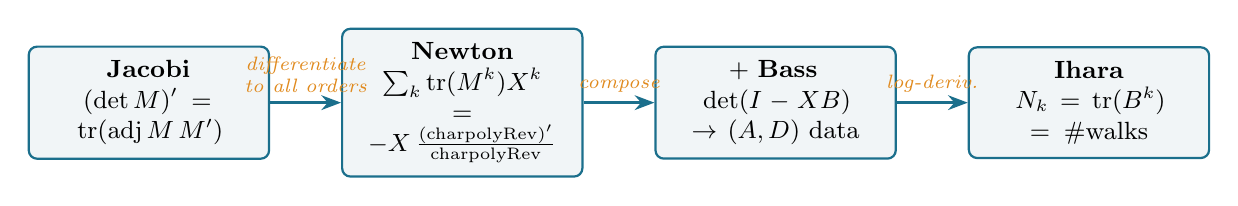
\begin{tikzpicture}[
  node distance=6mm and 9mm,
  box/.style={draw=ggteal,fill=ggband!40,rounded corners=3pt,line width=0.8pt,
    align=center,inner sep=5pt,text width=27mm,font=\small},
  arr/.style={-{Stealth[length=2.5mm]},ggteal,line width=0.9pt},
  lab/.style={font=\scriptsize\itshape,ggamber,align=center}]
\node[box] (jac) {\textbf{Jacobi}\\$(\det M)'=\tr(\adj M\,M')$};
\node[box,right=of jac] (new) {\textbf{Newton}\\$\sum_k\tr(M^k)X^k$\\$=-X\,\tfrac{(\charpolyRev)'}{\charpolyRev}$};
\node[box,right=of new] (bass) {\textbf{$+$ Bass}\\$\det(I-XB)$\\$\to(A,D)$ data};
\node[box,right=of bass] (nk) {\textbf{Ihara}\\$N_k=\tr(B^k)$\\$=\#$walks};
\draw[arr] (jac) -- node[lab,above]{differentiate\\to all orders} (new);
\draw[arr] (new) -- node[lab,above]{compose} (bass);
\draw[arr] (bass) -- node[lab,above]{log-deriv.} (nk);
\end{tikzpicture}
\caption{The spine of the paper. One elementary fact---a determinant's derivative is a
trace (Jacobi)---taken to all orders becomes the dictionary between a matrix's traces and its
characteristic polynomial (Newton), and composed with Bass's determinant formula reaches the closed
non-backtracking walk counts $N_k=\tr(B^k)$ of a graph. Each arrow is a theorem of this paper.}
\label{fig:spine}
\end{figure}

% ---------------------------------------------------------------
\section{Introduction: a short history, and why this paper}
\label{sec:intro}

\emph{Could a rule for differentiating a determinant---a fact so elementary it is often set as an
exercise---be the engine that, taken to all orders, recovers the characteristic polynomial from a
matrix's traces, and then counts the closed walks of a graph?} The answer is yes, and following it
requires three short histories to meet.

The first is \emph{Jacobi's formula}. In the nineteenth century Jacobi recorded how the determinant
of a matrix changes as its entries vary: $\mathrm{d}(\det M)=\tr(\adj M\cdot\mathrm{d}M)$, where
$\adj M$ is the adjugate (the transpose of the cofactor matrix). It is the matrix calculus behind
Liouville's formula for the Wronskian of a linear ODE, behind the Faddeev--LeVerrier algorithm that
computes a characteristic polynomial from traces, and behind every first-order perturbation of an
eigenvalue. It is also, in its \emph{algebraic} form---over an arbitrary commutative ring, with the
formal derivative of polynomials rather than a limit---absent from the largest formal library of
mathematics. Mathlib knew how to differentiate a determinant \emph{analytically}, as a smooth map
between normed spaces; it did not know the one-line algebraic identity.

The second is \emph{Newton's identities}. Newton related the power sums $p_k=\sum_i\lambda_i^k$ of a
collection of numbers to their elementary symmetric functions $e_k$---equivalently, the coefficients
of the polynomial $\prod_i(X-\lambda_i)$. Specialized to the eigenvalues of a matrix, the power sums
are exactly the traces $\tr(M^k)$, and the elementary symmetric functions are exactly the
coefficients of the characteristic polynomial. So Newton's identities, in this guise, are a bridge:
they let you compute the characteristic polynomial from the traces of powers, and conversely. Mathlib
has Newton's identities, but only in the abstract---for symmetric polynomials in free
variables---never connected to a matrix's traces. The bridge existed; its matrix end was missing,
recorded only at the very first coefficient as $\tr M=-\,(\text{next coefficient of the charpoly})$.

The third thread ties this to graphs, and to my earlier work. The Ihara zeta function of a graph
counts its closed non-backtracking walks; its reciprocal is the determinant $\det(I-XB)$ of
Hashimoto's non-backtracking operator $B$, and I formalized \emph{Bass's} reduction of that
determinant to vertex-sized data in a companion paper~\cite{IharaBass}. The counts $N_k=\tr(B^k)$ are
exactly the trace power sums that Newton's identity governs. The same derivative that powers Jacobi
and Newton therefore reaches, when applied to Bass's identity, all the way to the cycle counts of a
graph.

This paper formalizes that chain---Jacobi, then Newton, then the Ihara counts---in Lean~4, and is
exact about where the road, for now, ends.

% ---------------------------------------------------------------
\section{Jacobi's formula}
\label{sec:jacobi}

\emph{If you nudge one entry of a matrix, how does its determinant move---and why should the answer
involve the trace of anything?}

For a matrix $M$ whose entries are polynomials in a formal variable, write $M'$ for the entrywise
derivative and $\det M$ for the determinant (a polynomial). The answer is a trace.

\begin{theorem}[Jacobi's formula, in Lean~4]
\label{thm:jacobi}
For an $n\times n$ matrix $M$ of polynomials over a commutative ring,
\keyeq{(\det M)'\;=\;\tr\!\bigl(\adj M\cdot M'\bigr).}
The statement is \lean{sorry}-free (\lean{Matrix.derivative\_det});
\lean{\#print axioms} reports only \lean{propext}, \lean{Classical.choice}, \lean{Quot.sound}.
\end{theorem}

The proof is the determinant's own multilinearity, made one column at a time. Differentiating
$\det M=\sum_\sigma\varepsilon_\sigma\prod_i M_{\sigma(i),i}$ by the Leibniz rule and regrouping shows
that $(\det M)'$ is the sum, over columns $k$, of the determinant of $M$ with column $k$ replaced by
its derivative; Cramer's rule reads each of those single-column determinants off the adjugate, and
the sum reassembles as a trace. (In Lean the regrouping uses the product form of the Leibniz
formula, \lean{det\_apply'}, to keep every coefficient a genuine ring element rather than a signed
permutation---a small choice that makes the whole proof a chain of rewrites.)

\paragraph{Why this is useful, plainly.}
A determinant's derivative appears wherever a matrix moves. Three places it earns its keep:
\emph{Liouville's formula}---the Wronskian of a linear system evolves as
$\det(\Phi)'=\tr(A)\,\det(\Phi)$, which is Jacobi's formula for $\Phi'=A\Phi$; \emph{eigenvalue
perturbation}---the first-order change of a simple eigenvalue is a trace against its spectral
projection; and the \emph{Faddeev--LeVerrier algorithm}, which extracts a characteristic polynomial
and a matrix inverse from nothing but traces of powers, and whose correctness rests on exactly this
identity. Each is a theorem someone may one day wish to certify; each now has its first stone.

% ---------------------------------------------------------------
\section{The resolvent series: an eigenvalue-free engine}
\label{sec:resolvent}

\emph{Can one talk about $(I-XM)^{-1}$ without ever inverting anything---and without ever mentioning
an eigenvalue?}

Over formal power series, yes. The geometric series $\sum_k M^kX^k$ is an honest matrix of power
series, and it is the inverse of $I-XM$.

\begin{definition}[Resolvent series]
For an $n\times n$ matrix $M$ over a commutative ring, the \emph{resolvent series} is the matrix of
formal power series $\bigl(\,\sum_k M^k X^k\,\bigr)$, written \lean{resolventSeries M}.
\end{definition}

\begin{lemma}[The resolvent inverts $I-XM$, and its trace is the trace generating function]
\label{lem:resolvent}
\keyeq{(I-XM)\cdot\textstyle\sum_k M^kX^k\;=\;I,\qquad
   \tr\!\bigl(\textstyle\sum_k M^kX^k\bigr)\;=\;\sum_k \tr(M^k)\,X^k.}
Both are \lean{sorry}-free (\lean{one\_sub\_smul\_mul\_resolventSeries},
\lean{trace\_resolventSeries}). The inverse identity is proved from the fixed-point equation
$R=I+XM\!\cdot\!R$ by a single rearrangement---no eigenvalues, no algebraic closure, over any
commutative ring.
\end{lemma}

This is the engine of Section~\ref{sec:newton}. Its point is exactly its modesty: the standard way to
relate traces of powers to the characteristic polynomial passes through eigenvalues, and so needs the
matrix to split---an algebraically closed field, or a generic-matrix detour. The resolvent series
dispenses with all of it. The trace of $(I-XM)^{-1}$ is, by construction, the \emph{trace generating
function} $\sum_k\tr(M^k)X^k$, and that is the object Newton's identity is about.

\paragraph{Why this is useful, plainly.}
A formal resolvent is the natural home of any quantity one wants to read ``order by order'' in a
perturbation: the moments $\tr(M^k)$ of a matrix, the Green's function of a discrete operator, the
generating function of walks (Section~\ref{sec:walks}). Having $(I-XM)^{-1}$ available as certified
formal-power-series infrastructure---rather than re-deriving the geometric series each time---is a
small convenience that compounds.

% ---------------------------------------------------------------
\section{Newton's identity for matrix traces}
\label{sec:newton}

\emph{The traces $\tr(M),\tr(M^2),\dots$ and the coefficients of the characteristic polynomial are
two descriptions of the same matrix. What, exactly, is the dictionary between them?}

It is a single power-series identity, and it is Jacobi's formula taken to all orders. Write
$\charpolyRev M$ for the reversed characteristic polynomial $\det(I-XM)$---a polynomial with constant
term $1$, hence a unit in the power-series ring.

\begin{theorem}[Newton's identity for matrix traces, in Lean~4]
\label{thm:newton}
For an $n\times n$ matrix $M$ over a commutative ring, in the ring of formal power series,
\keyeq{(\charpolyRev M)'\;=\;-\,\charpolyRev M\cdot\sum_{k\ge0}\tr(M^{k+1})\,X^k.}
Equivalently $\sum_{k\ge1}\tr(M^k)X^k=-X\,(\charpolyRev M)'/\charpolyRev M$, the logarithmic
derivative. The statement is \lean{sorry}-free (\lean{Matrix.charpolyRev\_logDeriv}), over any
commutative ring, eigenvalue-free. At the linear coefficient it specializes to the lemma Mathlib
already had, $\tr M=-\,[\,X^1\,]\,\charpolyRev M$.
\end{theorem}

The proof is the chain promised in the introduction. Differentiate $\charpolyRev M=\det(I-XM)$ by
Jacobi (Theorem~\ref{thm:jacobi}); the derivative of $I-XM$ is $-M$, so $(\charpolyRev M)'$ is
$-\tr(\adj(I-XM)\cdot M)$. The adjugate of $I-XM$ is $\det(I-XM)$ times its inverse---which, by
Lemma~\ref{lem:resolvent}, is $\charpolyRev M$ times the resolvent series; the trace of the resolvent
against $M$ is the shifted generating function $\sum_k\tr(M^{k+1})X^k$. Transporting the polynomial
Jacobi identity along the coercion into power series and substituting closes the loop. The whole
argument never names an eigenvalue.

\paragraph{Why this is useful, plainly.}
This is the dictionary itself. Reading it one way, it computes the coefficients of the characteristic
polynomial---and hence the determinant, the trace, and (via Cayley--Hamilton) the inverse---from the
traces of powers; reading it the other way, it computes those traces from the polynomial. It is the
matrix-trace form of Newton's identities, the form a working mathematician actually meets, and the
form that Mathlib's symmetric-function version did not reach. The logarithmic-derivative shape
$\sum\tr(M^k)X^k=-X(\charpolyRev)'/\charpolyRev$ is, moreover, the universal pattern behind \emph{zeta
functions}: a determinant's reciprocal, log-differentiated, yields a count---which is precisely how
Section~\ref{sec:ihara} reaches the graph.

% ---------------------------------------------------------------
\section{Matrix powers count walks}
\label{sec:walks}

\emph{Before counting cycles, what does a single entry of $M^k$ count?}

The classical answer---walks---needs a formal home, and for \emph{directed} graphs Mathlib did not
have one. It records that a power of a \emph{simple} (undirected) graph's adjacency matrix counts
walks; the directed analogue, which the non-backtracking operator demands, was missing.

\begin{lemma}[Powers count walks]
\label{lem:walks}
For a matrix $M$ over a commutative semiring, the $(i,j)$ entry of $M^k$ is the sum, over
length-$k$ vertex walks from $i$ to $j$, of the product of the edge weights
(\lean{pow\_apply\_eq\_sum}). For the $0$--$1$ adjacency matrix of a decidable relation---a finite
directed graph---this is a genuine count: $\bigl((\text{adjacency})^k\bigr)_{ij}$ is the number of
length-$k$ directed walks from $i$ to $j$ (\lean{relMatrix\_pow\_apply}). Both are \lean{sorry}-free.
\end{lemma}

The trace then counts \emph{closed} walks, and---summing the diagonal---closed walks rooted at a
vertex. The same statement, reorganized over the cyclic index $\Z/(m{+}1)$, becomes a sum over
\emph{cyclic} walks (\lean{trace\_pow\_eq\_sum\_cyclicProd}), and the weight of a cyclic walk is
invariant under rotating its basepoint (\lean{cyclicProd\_comp\_finRotate}, and under the whole
rotation group). That rotation invariance is the door to geodesics---closed walks counted up to
cyclic rotation---though, as Section~\ref{sec:limits} is careful to say, only the door.

\begin{figure}[h]
\centering
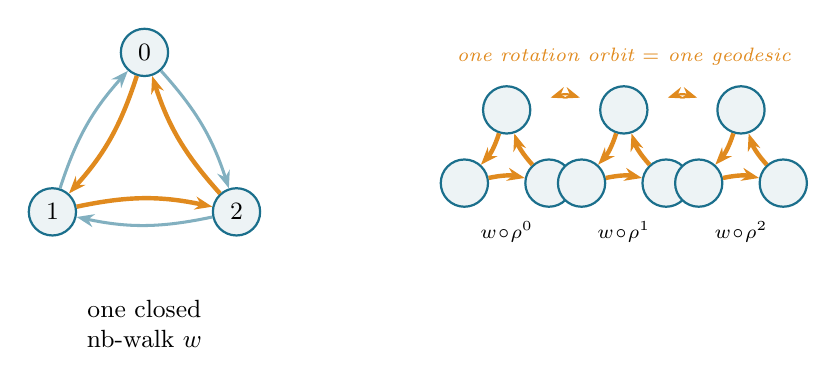
\begin{tikzpicture}[scale=1.0,
  v/.style={circle,draw=ggteal,fill=ggband!50,line width=0.8pt,inner sep=1.5pt,
    minimum size=6mm,font=\small},
  e/.style={-{Stealth[length=2.2mm]},line width=1.1pt},
  ee/.style={-{Stealth[length=2.2mm]},ggamber,line width=1.6pt}]
% triangle K3, the closed nb-walk 0->1->2->0 in amber
\node[v] (a) at (90:1.35) {$0$};
\node[v] (b) at (210:1.35) {$1$};
\node[v] (c) at (330:1.35) {$2$};
\draw[ee] (a) to[bend left=12] (b);
\draw[ee] (b) to[bend left=12] (c);
\draw[ee] (c) to[bend left=12] (a);
\draw[e,ggteal!55] (b) to[bend left=12] (a);
\draw[e,ggteal!55] (c) to[bend left=12] (b);
\draw[e,ggteal!55] (a) to[bend left=12] (c);
\node[font=\small,align=center] at (0,-2.1) {one closed\\nb-walk $w$};
% the orbit: three rotations -> one geodesic
\begin{scope}[xshift=4.6cm,scale=0.62]
  \foreach \k/\x in {0/0,1/2.4,2/4.8}{
    \node[v] (a\k) at ($(\x,0)+(90:1.0)$) {};
    \node[v] (b\k) at ($(\x,0)+(210:1.0)$) {};
    \node[v] (c\k) at ($(\x,0)+(330:1.0)$) {};
    \draw[ee] (a\k) to[bend left=12] (b\k);
    \draw[ee] (b\k) to[bend left=12] (c\k);
    \draw[ee] (c\k) to[bend left=12] (a\k);
    \node[font=\scriptsize] at (\x,-1.5) {$w\!\circ\!\rho^{\k}$};
  }
  \draw[{Stealth[length=2mm]}-{Stealth[length=2mm]},ggamber,line width=0.8pt]
    (0.9,1.25) to[bend left=18] (1.5,1.25);
  \draw[{Stealth[length=2mm]}-{Stealth[length=2mm]},ggamber,line width=0.8pt]
    (3.3,1.25) to[bend left=18] (3.9,1.25);
  \node[font=\scriptsize\itshape,ggamber,align=center] at (2.4,2.1)
    {one rotation orbit $=$ one geodesic};
\end{scope}
\end{tikzpicture}
\caption{Closed non-backtracking walks, and the rotation that groups them. \emph{Left:} the triangle
$K_3$ has six darts; one closed non-backtracking walk of length $3$ is shown in amber (the reverse
darts, in grey, would backtrack). \emph{Right:} rotating the basepoint by the cyclic shift
$\rho=\mathtt{finRotate}$ permutes the three rooted walks of this orbit while leaving the cyclic
weight fixed (\lean{cyclicProd\_comp\_finRotate})---so a single \emph{geodesic} accounts for an orbit
of rooted walks. Here $\tr(B^3)=6$: two orbits (the cycle and its reverse), three basepoints each.}
\label{fig:cyclic}
\end{figure}

\paragraph{Why this is useful, plainly.}
``Entry of a matrix power = number of walks'' is the workhorse of spectral graph theory: mixing
times, the method of moments for eigenvalue distributions, expander estimates, and the trace formulas
this paper composes all rest on it. Having it for \emph{directed} graphs, not only undirected ones,
is what lets the non-backtracking operator---an inherently directed object on oriented edges---be
counted at all.

% ---------------------------------------------------------------
\section{The Ihara counts, composed}
\label{sec:ihara}

\emph{If Jacobi differentiates a determinant into traces, and Bass collapses the Ihara determinant to
vertex data, what does their composition say?}

It says the non-backtracking counts of a graph are spectral. Let $B$ be Hashimoto's operator, $A$ the
adjacency and $D$ the degree matrix; Bass's formula~\cite{IharaBass} reads
$(1-X^2)^{|V|}\det(I-XB)=(1-X^2)^{|E|}\det(I-XA+X^2(D-I))$. Differentiating both sides
(Theorem~\ref{thm:jacobi}, on each determinant) and substituting Newton's identity
(Theorem~\ref{thm:newton}) on the non-backtracking side isolates the count generating function.

\begin{theorem}[The Ihara $N_k$ identity, in Lean~4]
\label{thm:ihara}
With $Q=\det(I-XA+X^2(D-I))$, in the power-series ring,
\keyeq{\sum_k\tr(B^{k+1})X^k\;=\;\frac{\det(I-XB)\,\bigl((1-X^2)^{|V|}\bigr)'-(1-X^2)^{|E|}Q'-Q\,\bigl((1-X^2)^{|E|}\bigr)'}{(1-X^2)^{|V|}\det(I-XB)}.}
The two $(1-X^2)$-powers and both determinants are units, so the division is the formal
$\mathtt{invOfUnit}$; the identity is \lean{sorry}-free (\lean{ihara\_Nk\_explicit}). It expresses the
non-backtracking counts $N_k=\tr(B^k)$ purely through the adjacency data $(A,D)$.
\end{theorem}

And the counts are combinatorial. Because $B$ is the $0$--$1$ adjacency matrix of the
non-backtracking relation on darts ($d\rightsquigarrow e$ when the head of $d$ is the tail of $e$ and
$e$ is not the reverse of $d$), Lemma~\ref{lem:walks} specializes:

\begin{theorem}[$\tr(B^k)$ counts non-backtracking walks, in Lean~4]
\label{thm:Nk}
\keyeq{\tr(B^k)\;=\;\#\{\text{closed non-backtracking walks of length }k,\ \text{rooted at a dart}\}.}
\lean{sorry}-free (\lean{trace\_hashimoto\_pow}).
\end{theorem}

So the same derivative that began as a one-line linear-algebra fact ends, four compositions later, as
the statement that a graph's non-backtracking walks of length $k$ number $\tr(B^k)$, and that this
number is computable from the graph's adjacency spectrum alone.

\paragraph{Why this is useful, plainly.}
Non-backtracking counts and spectra underpin sharp epidemic and percolation thresholds, spectral
community detection, and---through the Ihara analogue of the Riemann hypothesis---the very definition
of a Ramanujan graph as an optimal expander. Theorem~\ref{thm:ihara} certifies the bridge between
those counts and the adjacency data they are usually computed from; Theorem~\ref{thm:Nk} certifies
that the counts mean what they are said to mean.

\begin{table}[h]
\centering\small
\caption{Every machine-checked ingredient. All are \lean{sorry}-free; \lean{\#print axioms} reports
only \lean{[propext, Classical.choice, Quot.sound]}. Sources: \lean{Ihara/TraceFormula.lean} and
\lean{MathlibPR/MatrixWalkCount.lean}.}
\label{tab:results}
\begin{tabular}{@{}llc@{}}
\toprule
\textbf{Lean name} & \textbf{Statement} & \textbf{\S}\\
\midrule
\lean{Matrix.derivative\_det} & $(\det M)'=\tr(\adj M\cdot M')$ (Jacobi) & \ref{sec:jacobi}\\
\lean{one\_sub\_smul\_mul\_resolventSeries} & $(I-XM)\sum_k M^kX^k=I$ & \ref{sec:resolvent}\\
\lean{trace\_resolventSeries} & $\tr\sum_k M^kX^k=\sum_k\tr(M^k)X^k$ & \ref{sec:resolvent}\\
\lean{Matrix.charpolyRev\_logDeriv} & $(\charpolyRev M)'=-\charpolyRev M\sum_k\tr(M^{k+1})X^k$ (Newton) & \ref{sec:newton}\\
\lean{pow\_apply\_eq\_sum} & $(M^k)_{ij}=\sum_{\text{walks}}\prod(\text{weights})$ & \ref{sec:walks}\\
\lean{relMatrix\_pow\_apply} & directed walk count, $0$--$1$ case & \ref{sec:walks}\\
\lean{trace\_pow\_eq\_sum\_cyclicProd} & $\tr(M^{m+1})=\sum_{\text{cyclic }w}\text{cyclicProd}$ & \ref{sec:walks}\\
\lean{cyclicProd\_comp\_finRotate\_iterate} & rotation invariance (full group) & \ref{sec:walks}\\
\lean{ihara\_Nk\_explicit} & $\sum_k\tr(B^{k+1})X^k$ from $(A,D)$ & \ref{sec:ihara}\\
\lean{trace\_hashimoto\_pow} & $\tr(B^k)=\#$ closed nb-walks & \ref{sec:ihara}\\
\bottomrule
\end{tabular}
\end{table}

\begin{table}[h]
\centering\small
\caption{Independent numerical cross-checks (\texttt{SymPy}), exact symbolic equality. The graph row
is the triangle $K_3$: the trace of $B^k$ matches a brute-force enumeration of rooted closed
non-backtracking walks, $0,0,6,0,0,6$ for $k=1,\dots,6$ (the cycle and its reverse, three basepoints
each).}
\label{tab:checks}
\begin{tabular}{@{}lll@{}}
\toprule
\textbf{Identity} & \textbf{Instance} & \textbf{Result}\\
\midrule
Jacobi $(\det M)'=\tr(\adj M\,M')$ & $3\times3$ matrix of polynomials & exact\\
Newton (log-derivative) & $3\times3$ and $2\times2$, mod $X^8$ & exact\\
$\tr(B^k)=\#\{\text{rooted nb-walks}\}$ & $K_3$, $k=1,\dots,6$ & $0,0,6,0,0,6$ both\\
Bass $(1{-}u^2)^{|V|}\det(I{-}uB)=\dots$ & $K_3$ & exact\\
\bottomrule
\end{tabular}
\end{table}

% ---------------------------------------------------------------
\section{What I claim, and what I do not}
\label{sec:limits}

The mathematics is classical throughout: Jacobi's formula, Newton's identities, the walk count, and
Bass's theorem are all old. The contribution is the formalization, and I separate the two on purpose.

\paragraph{What I claim as new (as formalization).}
(N1) the first machine-checked proof I am aware of, in any proof assistant, of Jacobi's
\emph{algebraic} formula $(\det M)'=\tr(\adj M\cdot M')$; (N2) the \emph{matrix-trace} form of
Newton's identities, $(\charpolyRev M)'=-\charpolyRev M\sum_k\tr(M^{k+1})X^k$, which Mathlib had only
at the linear coefficient; (N3) the resolvent series $(I-XM)^{-1}=\sum_k M^kX^k$ and the
\emph{directed}-graph walk count, neither in the library. All are formalization contributions; none
is new mathematics.

\paragraph{And, plainly, what this is not.}
$\tr(B^k)$ counts \emph{rooted} closed non-backtracking walks---walks with a chosen basepoint
dart---\emph{not} closed geodesics, which are the cyclic equivalence classes of such walks, and not
the prime geodesics whose Euler product is the analytic Ihara zeta. The cyclic structure that
distinguishes them \emph{is} set up here: the trace is rewritten as a sum over cyclic walks, and the
weight is proved invariant under the whole rotation group, so each weight is a class function on the
rotation orbits. But the orbit-counting, the primitive-period bookkeeping, the M\"obius inversion,
and the Euler product that turn rooted counts into prime-geodesic counts are \emph{not} built. I have
laid the combinatorial floor; the number-theoretic superstructure is mapped, not raised.

% ---------------------------------------------------------------
\section{Implications}
\label{sec:implications}

Three kinds, in decreasing order of how firmly I can claim them, and a methodological aside.

\paragraph{Reusable, certified building blocks.}
Jacobi's algebraic formula, the resolvent series, the matrix-trace Newton identity, and the directed
walk count are now machine-checked and available to anyone formalizing characteristic polynomials,
the Faddeev--LeVerrier algorithm, zeta functions of graphs, or expander spectra. Mathlib had none of
the four in usable form. This is the implication I can state most firmly, and the one I would point a
future formalizer to first.

\paragraph{A foothold for what these unlock.}
Newton's identity is the gateway to computing characteristic-polynomial coefficients from traces and
back; Jacobi underlies Faddeev--LeVerrier and Liouville's formula; the Ihara composition is one step
from the prime-geodesic counting it sets up. Each is a landmark these stones could support.

\paragraph{The mathematics, with a note of caution.}
These identities matter because the objects downstream of them---characteristic polynomials,
non-backtracking spectra, Ramanujan expanders---matter. I am wary of borrowing that importance:
certifying a foundational identity ships no algorithm and no network. Its value is in certified
foundations and in the growing corpus of formalized mathematics, not in immediate application; I
claim the former, not the latter.

\paragraph{A methodological aside.}
This development was carried out with an AI system as a research instrument: it proposed definitions,
lemmas and tactics, and a build-as-oracle loop verified or rejected each against the kernel. The
careful accounting here---every claim sized to exactly what was proved, the rooted-versus-geodesic
distinction drawn as sharply as the theorems---is part of what I hope the work shows: that
AI-assisted formalization can resist the over-claiming the method invites, precisely because the
proof assistant, not the assistant, has the last word.

% ---------------------------------------------------------------
\section{Where this stops being useful}
\label{sec:context}

Honesty cuts both ways, so the limits are stated as plainly as the results. Theorem~\ref{thm:ihara}
is a \emph{generating-function} identity, not the analytic zeta; it locates no pole and names no
prime. Theorem~\ref{thm:Nk} counts \emph{rooted} walks, and the gap to geodesics---an entire
necklace-counting and M\"obius-inversion theory---is real, not cosmetic. Newton's identity is proved
over a commutative ring but says nothing about when the characteristic polynomial \emph{splits};
Jacobi is for matrices of polynomials, and the smooth-manifold version remains a separate object.
This paper is a handful of certified stones near the start of a long road, and I would rather name
the road than overstate the stones.

% ---------------------------------------------------------------
\section{Related work}
\label{sec:related}

The mathematics is classical: Jacobi's formula and Liouville's, Newton's identities and the
Faddeev--LeVerrier algorithm built on them, the walk-counting reading of matrix powers, and---for the
application---Ihara's zeta function~\cite{Ihara1966}, Hashimoto's edge operator~\cite{Hashimoto1989},
Bass's determinant formula~\cite{Bass1992}, and Terras's modern account~\cite{Terras2011}. On the
formalization side, Mathlib~\cite{Mathlib2020} provides determinants, the adjugate, Cramer's rule,
the reversed characteristic polynomial (at the linear coefficient only), Newton's identities for
symmetric polynomials, and walk counts for simple graphs---but not Jacobi's algebraic formula, the
matrix-trace Newton identity, the resolvent series, or the directed walk count. This development is a
companion to my earlier Lean formalizations of the matching polynomial~\cite{PartI,PartII} and of
Bass's formula~\cite{IharaBass}; I am not aware of a prior machine-checked proof of Jacobi's
algebraic formula or of the matrix-trace Newton identity in any proof assistant.

% ---------------------------------------------------------------
\section{Conclusion}

I set out from the most elementary fact I could name---how a determinant moves when its matrix
moves---and followed it, in a proof assistant, through Newton's dictionary between traces and
characteristic polynomials, and on to the closed-walk counts of a graph. None of this is new
mathematics; the contribution is that Jacobi's algebraic formula, the matrix-trace Newton identity,
the resolvent series, and the directed walk count are now machine-verified where I could find no
prior formalization, and that they compose, all the way to the Ihara counts. The prime-geodesic
counting they set up, and full spectral generality, remain ahead---mapped, but unraised. I offer this
as a pearl and an invitation.

\paragraph{Artifacts.} All Lean sources (\lean{sorry}-free, depending only on the three standard
axioms), are available at
\begin{center}
\url{https://github.com/karlesmarin/godsil-gutman-lean}
\end{center}
in \lean{Ihara/TraceFormula.lean} (Jacobi, Newton, the Ihara composition) and
\lean{MathlibPR/MatrixWalkCount.lean} (the resolvent series, the walk count, the cyclic structure).
Verify the axiom footprint with, e.g., \lean{\#print axioms Matrix.charpolyRev\_logDeriv}
$\rightsquigarrow$ \lean{[propext, Classical.choice, Quot.sound]}.

\begin{thebibliography}{99}
\bibitem{Bass1992} H.~Bass, \emph{The Ihara--Selberg zeta function of a tree lattice}, Internat. J.
  Math. \textbf{3} (1992), 717--797.
\bibitem{Hashimoto1989} K.~Hashimoto, \emph{Zeta functions of finite graphs and representations of
  $p$-adic groups}, in \emph{Automorphic forms and geometry of arithmetic varieties}, Adv. Stud. Pure
  Math. \textbf{15} (1989), 211--280.
\bibitem{Ihara1966} Y.~Ihara, \emph{On discrete subgroups of the two by two projective linear group
  over $\mathfrak{p}$-adic fields}, J. Math. Soc. Japan \textbf{18} (1966), 219--235.
\bibitem{Mathlib2020} The mathlib Community, \emph{The Lean mathematical library}, in \emph{Proc. 9th
  ACM SIGPLAN Int. Conf. on Certified Programs and Proofs (CPP 2020)}, 367--381.
\bibitem{PartI} C.~Mar\'in, \emph{Random Signs into Matchings: a machine-checked Godsil--Gutman
  identity in Lean~4} (2026).
\bibitem{PartII} C.~Mar\'in, \emph{Unfolding a Graph into a Tree: Heilmann--Lieb real-rootedness in
  Lean~4} (2026).
\bibitem{IharaBass} C.~Mar\'in, \emph{Folding Edges into Vertices: a machine-checked proof of Bass's
  determinant formula for the Ihara zeta in Lean~4} (2026), Zenodo DOI
  \texttt{10.5281/zenodo.20573120}.
\bibitem{Terras2011} A.~Terras, \emph{Zeta Functions of Graphs: A Stroll through the Garden},
  Cambridge Studies in Advanced Mathematics \textbf{128}, Cambridge Univ. Press, 2011.
\end{thebibliography}

\end{document}
